\documentclass{standalone}
\usepackage{tikz} % Import the tikz package
\usetikzlibrary{automata} % Import library for drawing automata
\usetikzlibrary{positioning} % ...positioning nodes
\usetikzlibrary{arrows} % ...customizing arrows
\tikzset{node distance=2.5cm,
    every state/.style={
        semithick,
        fill=gray!10},
    initial text={},
    double distance=2pt,
    every edge/.style={
        draw,
        ->,>=stealth',
        auto,
        semithick}}
\let\epsilon\varepsilon
\begin{document}
    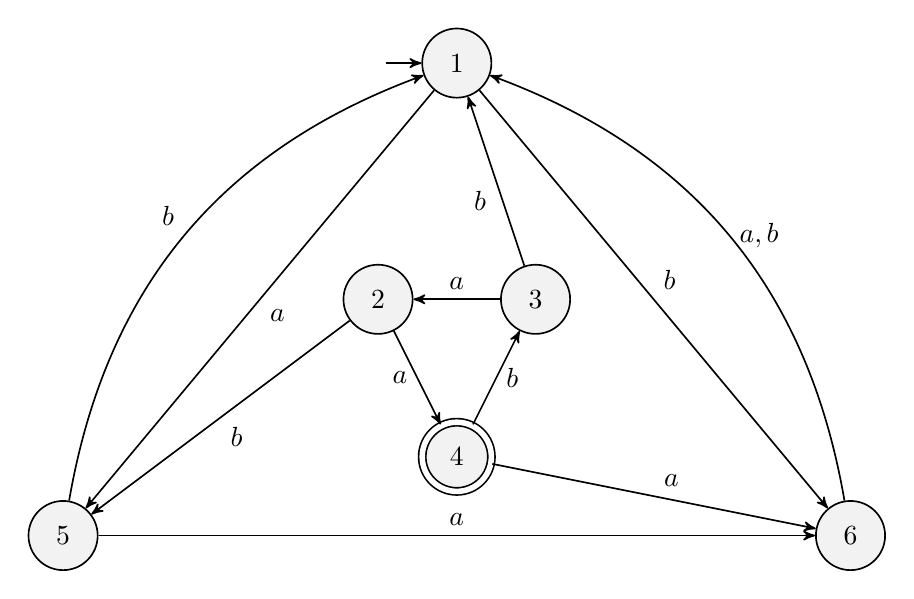
\begin{tikzpicture}
        \node[initial,state] (1) at (0,4) {1};
        \node[state] (2) at (-1,1) {$2$};
        \node[state] (3) at (1,1) {$3$};
        \node[state,accepting] (4) at (0,-1) {$4$};
        \node[state] (5) at (-5,-2) {$5$};
        \node[state] (6) at (5,-2) {$6$};

        \draw (1) edge[] node {$a$} (5);
        \draw (1) edge[] node {$b$} (6);
        
        \draw (2) edge[left] node {$a$} (4);
        \draw (2) edge[] node {$b$} (5);
        
        \draw (3) edge[above] node {$a$} (2);
        \draw (3) edge[] node {$b$} (1);

        \draw (4) edge[] node {$a$} (6);
        \draw (4) edge[right] node {$b$} (3);

        \draw (5) edge[] node {$a$} (6);
        \draw (5) edge[bend left] node {$b$} (1);

        \draw (6) edge[bend right,right] node {$a,b$} (1);
    \end{tikzpicture}
\end{document}